\documentclass[11pt,a4paper]{article}
\usepackage[utf8]{inputenc}
\usepackage[spanish]{babel}
\usepackage[pdftex]{graphicx}
\usepackage{color}
\usepackage{pdfpages}
\usepackage{url}

\title{Práctica Nagios}
\author{Palbo Jiménez Mateo y Mihaita Alexandru Lupoiu}
\date{Diciembre 2014}

\begin{document}

\maketitle
\tableofcontents
\clearpage

\section{Introducción a Nagios}

    Nagios es un sistema de monitorización de redes ampliamente utilizado, de código abierto, que vigila los equipos (hardware) y servicios (software) que se especifiquen, alertando cuando el comportamiento de los mismos no sea el deseado. Entre sus características principales figuran la monitorización de servicios de red (SMTP, POP3, HTTP, SNMP...), la monitorización de los recursos de sistemas hardware (carga del procesador, uso de los discos, memoria, estado de los puertos...), independencia de sistemas operativos, posibilidad de monitorización remota mediante túneles SSL cifrados o SSH, y la posibilidad de programar plugins específicos para nuevos sistemas\cite{nagios-wikipedia}.
    
\begin{figure}[hbtp]
\centerline{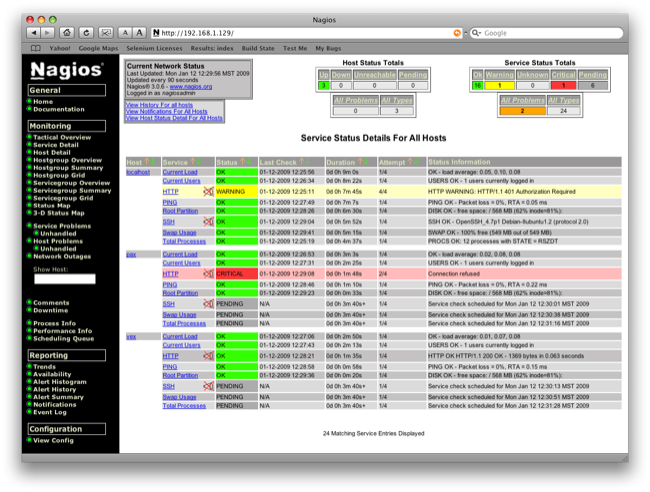
\includegraphics[width=9cm]{nagios3-1.png}}
\caption{Interfaz de Nagios}
\label{figura1}
\end{figure}    

    Se trata de un software que proporciona una gran versatilidad para consultar prácticamente cualquier parámetro de interés de un sistema, y genera alertas, que pueden ser recibidas por los responsables correspondientes mediante (entre otros medios) correo electrónico y mensajes SMS, cuando estos parámetros exceden de los márgenes definidos por el administrador de red.

    Nagios\cite{web} fue originalmente diseñado para ser ejecutado en GNU/Linux, pero también se ejecuta bien en variantes de Unix.

    Nagios está licenciado bajo la GNU General Public License Version 2 publicada por la Free Software Fundation.
    
    Algunas de las características que Nagios tiene son:
\begin{itemize}

\item Monitoréo de Servicios de Red
\item Monitoreo de Host y sus recursos como CPU, Memoria, Discos, etc
\item Desarrollo de Plugins para el chequeo de una infinidad de plataformas y servicios
\item Capacidad de Services Checks en paralelo
\item Capacidad de Definir Host/Servicios padres o hijos, lo que permite detectar el origen del problema en caso de no ser de la propia máquina (Ejemplo: la caída de un server por la falla de un Switch)
\item Definición de Contactos para el envío de notificaciones
\item Capacidad de definir manejadores de eventos para el manejo de eventos de manera proactiva
\item Log de eventos
\item Interface Web para la visualización de estados de servicio, históricos, Archivo de Log, etc
\item Integración con herramientas que la comunidad ha desarrollado
\item Multiplataforma, aunque fue desarrollado originalmente para correr sobre Linux

\end{itemize}

Que es lo que se gana con Nagios.
\begin{itemize}
\item Supervisión Continua de la plataforma de TI
\item Esto te permite mejorar los tiempos de disponibilidad de los servicios
\item Alertar al equipo de TI ante alertas preventivas (Warning) o críticas (Critical)
\item Reaccionar de manera preventiva y no reactiva ante los eventos que nagios detecte.
\item Aumenta la productividad de las TIC
\item Generar Reportes de los eventos.
\item Planificar mantencion de tu hardware o servicios.
\item Planificar el cambio o renovación de la Infraestructura de TIC
\end{itemize}    

    Además de Nagios existen otras alternativas como por ejemplo: 

    
\section{Funcionamiento de Nagios}

Explicación de cómo funciona Nagios

Se pueden incluir figuras como por ejemplo la Figura~\ref{figura1} de la página \pageref{figura1}

\begin{figure}
\centerline{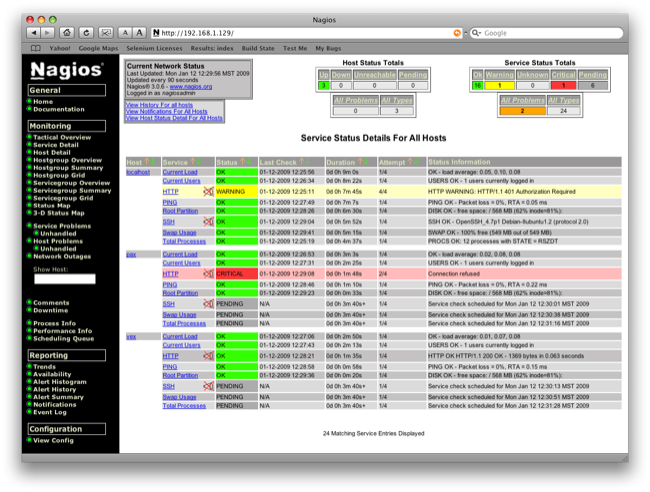
\includegraphics[width=6cm]{nagios3-1.png}}
\caption{Figura de ejemplo}
\label{figura1}
\end{figure}

\section{Instalación de Nagios}

Se explica cómo instalar Nagios. Sería conveniente que supiéseis instalar Nagios tanto utilizando
la distribución de paquetes del sistema operativo como a partir de los códigos fuente.

\section{Acceso a Nagios mediante el navegador}

Se debe explicar cómo se debe configurar el servidor web para acceder a Nagios a través del navegador
y  tambíen la interfaz web que presenta Nagios.

\section{Configurar Nagios}

Se debe explicar los distintos ficheros de configuración de Nagios y cómo se configuran para 
monitorizar tanto al sistema local como a sistemas remotos.

\section{Experiencia de instalación y configuración de  Nagios}

Se deben detallar los pasos que se han seguido para la instalación y configuración de Nagios
tanto para monitorizar el sistema local como sistemas remotos.

\begin{thebibliography}{1}

\bibitem{web} Página web del proyecto de Nagios: \url{http://www.nagios.org}
\bibitem{nagios-wikipedia} Wikipedia Nagios: \url{http://es.wikipedia.org/wiki/Nagios}
\bibitem{nagios-wikipedia} Página web del proyecto de OpenNMS: \url{http://www.opennms.org/wiki/Main_Page}
\bibitem{nagios-wikipedia} Página web del proyecto de Pandorafms: \url{http://pandorafms.com/}
\bibitem{nagios-wikipedia} Página web del proyecto de NeDi: \url{http://www.nedi.ch/}

\end{thebibliography}

\end{document}
